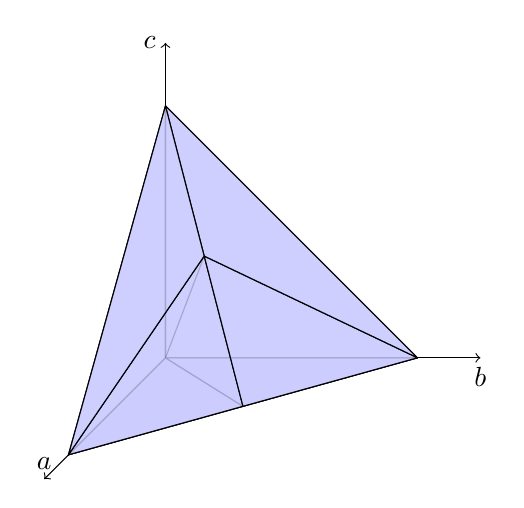
\begin{tikzpicture}[join=round,scale=0.8]
    \tikzstyle{conefill} = [fill=blue!20,fill opacity=0.8]
    \tikzstyle{ann} = [fill=white,font=\footnotesize,inner sep=1pt]
    \tikzstyle{ghostfill} = [fill=white]
    \tikzstyle{ghostdraw} = [draw=black!50]
    
    \draw[arrows=->,line width=.4pt](0,0,0)--(0,0,5); %Z_achse
    \draw[arrows=->,line width=.4pt](0,0,0)--(0,5,0); %Y-ACHSE
    \draw[arrows=->,line width=.4pt](0,0,0)--(5,0,0); %X-ACHSE
    %\draw[arrows=<-,line width=.4pt](.42,-.767)--(4,-2);
    
    \path (5,0,0) node[below] {$b$} (0,0,5) node[above] {$a$} (0,5,0) node[left] {$c$};
   
% erste Koordinate ist B!!! 
% zweite Koordinate ist C!!!   
% dritte Koordinate ist A!!!


% äußere Flächen!

\filldraw[conefill](0,0,0)--(0,4,0)--(0,0,4)--cycle;
\filldraw[conefill](0,0,0)--(4,0,0)--(0,0,4)--cycle;
\filldraw[conefill](0,0,0)--(4,0,0)--(0,4,0)--cycle;

% untenfläche
\filldraw[conefill](0,0,0)--(0,0,4)--(2,0,2)--cycle;
\filldraw[conefill](0,0,0)--(4,0,0)--(2,0,2)--cycle;

%
\filldraw[conefill](0,0,4)--(2,0,2)--(1,2,1)--cycle;
\filldraw[conefill](4,0,0)--(2,0,2)--(1,2,1)--cycle;

\filldraw[conefill](4,0,0)--(1,2,1)--(0,4,0)--cycle;
\filldraw[conefill](0,0,4)--(1,2,1)--(0,4,0)--cycle;

% zur Übersichtlichkeit die gerade im "inneren" des Cones
\draw [opacity=0.2] (0,0,0) -- (1,2,1) ;
\end{tikzpicture}